\section{Introduction}

\subsection{Objet du projet}

Le but de ce projet est d’améliorer le système d’information du domaine \emph{gestion de matériel} de l’entreprise GSTP.

L’objectif de ce projet étant une étude préalable, nous nous limiterons aux phases de spécifications et de conception du système d’information. Nous ne prendrons pas en charge les phases suivants l’étude préalable, c’est à dire : l’étude détaillée, la réalisation..

\subsection{Contexte général du projet}
GSTP est une entreprise de travaux, spécialisée dans le terrassement et le génie civil.
Ceci représente une quarantaine de chantiers, répartis sur un rayon de 500 km.
Au niveau de l’organisation de l’entreprise, sa structure est logiquement divisée en plusieurs services :
\begin{itemize}
    \item Direction Générale (DG)
    \item Direction des ressources humaines (DRH)
    \item Direction des finances et comptabilité (DFC)
    \item Direction informatique (DI)
    \item Direction du matériel (DM)
    \item Direction travaux, études et méthodes (DTEM)
\end{itemize}
La direction des travaux, études et méthodes supervise les chantiers. Chaque chantier est autonome en fonctionnement et financièrement. Ainsi les besoins en matériels sont gérés par la direction des matériels. C’est une relation client-fournisseur interne à l’entreprise.

Nous nous intéresserons plus particulièrement a la direction matériel et ses départements. La DM est attachée à la Direction Générale et a pour missions :
\begin{itemize}
    \item Affecter le matériel au chantier
    \item Assurer la maintenance et la rénovation du matériel
    \item Acquérir de nouveaux matériels
    \item Gérer le stock de pièces de rechange
    \item Louer/Facturer aux chantiers, l’utilisation du matériel
\end{itemize}
Pour gérer l’ensemble de ses départements, la direction matériel utilise de nombreuses applications (obsolètes) de gestion et de planification :
\begin{itemize}
    \item Département Matériel :
        \subitem Gestion de planning
        \subitem Facturation
    \item Département maintenance:
        \subitem Gestion de stocks de pièces de rechange
        \subitem Planification de la maintenance
    \item Département achat :
        \subitem Gestion des fournisseurs
        \subitem Gestion des bons de commande
\end{itemize}


Ces applications sont indépendantes les unes des autres et ne sont intégrées dans aucun système d’information.

\section{Livrables}

Lors de la phase d’étude préalable, des livrables bien définis doivent être fournis aux clients. Ces derniers sont remis lors d’étapes spécifiques présentées ci-après.  L’objet de cette partie est de décrire le rôle et le contenu de chacun des ces livrables.
\subsection{Initialisation et Organisation du projet}

A l’initialisation, deux documents doivent être rédigés. Lors de cette étape, il ne s’agit pas de chercher des solutions informatiques, mais de définir le cadre dans lequel nous nous attacherons à évoluer :

\begin{itemize}
    \item Document d’initialisation : ce document décrit notre démarche pour réaliser le projet, il présente les informations suivantes :
    \begin{itemize}
        \item présentation du contexte global et des objectifs clients.
        \item les livrables attendus
        \item le mode opératoire et le phasage
        \item définition des tâches et planning,
        \item l’organisation de l’équipe
        \item l’analyse des risques
    \end{itemize}
    \item Plan d’assurance qualité : ce document décrit la mise en place de la politique qualité dans le contexte du projet. Il contient :
    \begin{itemize}
        \item la description des documents (dont les livrables) sur le plan de la mise en forme
        \item le cycle de vie des documents
        \item les ressources et outils
        \item les modalités de validations internes et de recette
        \item un annexe (contenant des parties de documents types ou des modèles)
    \end{itemize}
\end{itemize}

\subsection{Expression des besoins}

Cette étape doit être réalisée en interaction avec le client. Il s’agit de comprendre ses attentes afin de les reformuler dans un document : le dossier d’expression des besoins.

Il contient :
\begin{itemize}
    \item une présentation du contexte du projet (approche métier),
    \item les éventuelles orientations stratégiques de la MOA
    \item une analyse de l’existant (dont le SI)
    \item la cible fonctionnelle (modèle de référence des activités et processus de l’entreprise).
    \item les écarts avec l’existant (les dysfonctionnements)
    \item les attentes des partenaires
    \item le benchmarking
    \item les thèmes de progrès
\end{itemize}

\subsection{Construction des scénarios}

Un unique document sera fourni. Dans ce rapport, deux scénarios de mise en œuvre seront envisagés : une solution spécifique et une solution standard de type ERP.

Le document contiendra pour chaque scénario la démarche préconisée :
\begin{itemize}
    \item la nouvelle organisation
    \item l’architecture technique
    \item l’architecture applicative
    \item l’architecture logicielle
\end{itemize}
\subsection{Évaluation des scénarios}

Les deux scénarios présentés dans la partie précédente doivent ensuite être évalués et comparés afin de choisir celui que nous adopterons. Un livrable explicitant notre choix sera fourni, il doit permette au client de comprendre en quoi la solution choisie répond le mieux à son besoin.

Pour chaque scénario, on va rassembler les éléments de choix, à savoir les points forts et les points faibles.


\subsection{Restitution}

C’est la dernière étape, un dossier bilan doit être livré. Le projet est également présenté oralement durant un rendez-vous client.

Durant la présentation finale (powerpoint), nous exposerons notre démarche, présenterons les deux solutions et expliquerons les raisons de notre choix. Il s’agira de convaincre en mettant en avant les points forts de notre projet.

En ce qui concerne le dossier bilan, il vient conclure la phase d’étude préalable. Il souligne :
\begin{itemize}
    \item les évolutions majeures apportées au produit livré par rapport à la définition présentée dans le dossier d’initialisation.
    \item le plan de charges est actualisé, il met en avant les écarts et explique l’origine de ces écarts.
    \item une  synthèse des difficultés rencontrées.
\end{itemize}

Un certain nombre de documents de suivi sont également réalisé tout au long du projet. Il sont cités ici à titre indicatif car il ne s’agit pas de livrables :
\begin{itemize}
    \item Fiche de suivi d’avancement des livrables intermédiaires
    \item Journal de réunion
    \item Fiche de suivi individuel par séance
    \item Fiche de suivi global par séance
    \item Tableau de bord
\end{itemize}

\section{Mode opératoire et phasage}

\subsection{Choix de la méthode}

Afin de réaliser cette étude préalable, nous avons opté pour la méthode MERISE, simplement parce qu'elle permet une décomposition du système d'information de l'entreprise en domaines et processus facilement analysables et donc utiles pour notre étude préalable. Nous capitalisons aussi sur le fait que l’existant est basé sur ce modèle.

\subsection{Phases}

Pour Chaque phase, nous préciserons son but, son déroulement et le(s) livrable(s) attendu(s). Les phases de notre étude préalable sont les suivantes :

\subsubsection{Initialisation}

\paragraph{Buts}
\begin{itemize}
    \item Cibler le champs d’étude du projet
    \item Identifier les contraintes et risques
    \item Élaborer notre démarche
    \item Élaborer un plan d’assurance qualité
\end{itemize}


\paragraph{Déroulement}
\begin{description}
    \item[Contexte général]{
        Il s’agit de faire une introduction présentant brièvement l’entreprise, l’état du service existant, ainsi que notre rôle dans ce projet.
    }
    \item[Livrables]{
        Il s’agit d’élaborer une liste exhaustive des livrables.
    }
    \item[Mode opératoire et phasage]{
        Il s’agit de choisir les méthodes à adopter, découper le projet en plusieurs phases.
    }
    \item[Activités / taches]{
        Il s’agit d’identifier les taches et activités de chaque phase, les répartir entre les différents collaborateurs selon un planning prévisionnel.
    }
    \item[Organisation de l’équipe]{
        Il s’agit de définir le rôle de chaque membre ainsi que ses principales missions au sein du projet.
    }
    \item[Analyse des risques]{
        Il s’agit de faire une analyse prévisionnelle des risques liés au projet et élaborer un plan de gestion de ces risques.
    }
\end{description}

\paragraph{Livrables}
\begin{itemize}
    \item Dossier d’initialisation
    \item Plan d'Assurance Qualité
\end{itemize}

\subsubsection{Expression des besoins}

\paragraph{But}
\begin{itemize}
    \item Identifier les thèmes de progrès pour restreindre les futurs scénarios tout en répondant au mieux aux attentes du client.
\end{itemize}


\paragraph{Déroulement}
\begin{description}
    \item[Contexte du projet dans l’entreprise GSTP]{
        comprendre le modèle métier de l'entreprise, identifier les activités , les directions et services concernés par le projet ainsi que les processus stratégiques à analyser.
    }
    \item[Analyse de l’existant]{
        étudier l’existant organisationnel et informatique afin d’identifier les écarts par rapport à la stratégie de l’entreprise ainsi que les processus à modifier. 
    }

    \item[Normes et benchmarking]{
        cette étape consiste à se renseigner sur les différentes normes et benchmarks existants, mais aussi au près des concurrents afin de comprendre leur méthode, identifier les avantages qu’ils en tirent.  Le but final étant de retenir les “best practice”.
    }

    \item[Cible de référence]{
        il faut élaborer un modèle de référence des processus de l’entreprise à partir des dysfonctionnements relevés, des “best practice” retenue, des attentes clients,..  et indépendamment  des moyens organisationnels et informatiques.
    }

    \item[Thèmes de progrès]{
        identifier les axes d’amélioration.
    }
\end{description}

\paragraph{Livrables}
\begin{itemize}
    \item Dossier d’expression des besoins (EB)
\end{itemize}

\subsubsection{Analyse et conception des solutions informatiques et organisationnelles}

\paragraph{Buts}
\begin{itemize}
    \item[Proposer deux solutions distinctes]{
        l’une étant spécifique (construite de A à Z, pour répondre le plus précisément possible aux besoins), l’autre plus standard (basé sur des systèmes standards de type ERP, qui seront adaptés au besoin).
    }
\end{itemize}


\paragraph{Déroulement}
\begin{itemize}
    \item Analyse et conception
        \subitem Définitions des stratégies d’informations
        \subitem Analyse générale de l’architecture applicative cible
        \subitem Conception générale de l’architecture applicative cible
    \item Démarche pour la mise en place d’une solution spécifique
        \subitem Analyse des impacts organisationnels
        \subitem Analyse des impacts informatiques (architectures technique, applicative, logicielle).
    \item Analyse  des solutions existantes du marché/Choix d’une solution :
        \subitem Analyse des impacts organisationnels
        \subitem Analyse des impacts informatiques (architectures technique, applicative, logicielle).
\end{itemize}

\paragraph{Livrables}
\begin{itemize}
    \item Dossier de description des scénarios
\end{itemize}

\subsubsection{Évaluation des scénarios}

\paragraph{Buts}
\begin{itemize}
    \item Évaluer les différents scénarios et en faire ressortir les avantages et inconvénients de chacun afin de construire une étude comparative..
    \item Choisir la solution qui nous semble la plus adaptée aux besoins du clients.
\end{itemize}

\paragraph{Déroulement}
\begin{itemize}
    \item Évaluation des solutions : il s’agit de comparer les deux scénarios et d’en voir les différences. Une présentation des avantages/inconvénients de ces scénarios semble intéressante à produire.
    \item Choix
\end{itemize}

\paragraph{Livrables}
\begin{itemize}
    \item Dossier de choix
\end{itemize}

\section{Identification des activités et des tâches}

Pour planifier l’étude préalable, il est fondamentale d’identifier l’ensemble des activités et les tâches qui y sont associées. Celles que nous avons identifié sont :
\begin{itemize}
    \item Suivi de projet : {\bf A1}
        \subitem Organisation
        \subitem Planification
        \subitem Évaluation
        \subitem Pilotage/Suivi

    \item Gestion/Contrôle de documents : {\bf A2}
        \subitem Diffusion PAQ
        \subitem Respect PAQ
        \subitem Validation des livrables
        \subitem Organisation des réunions internes
        \subitem Organisation des rencontres avec le client

    \item Production : {\bf A3}
        \subitem Élaboration des livrables
        \subitem Réalisation des rapports
        \subitem Mise en commun des informations
\end{itemize}

Pour représenter l’ordonnancement des tâches, nous allons utilisé un diagramme de GANT (fait avec MS Project) qui montrera le positionnement des tâches sur l’échelle du temps et l’utilisation des ressources (membres du projet).

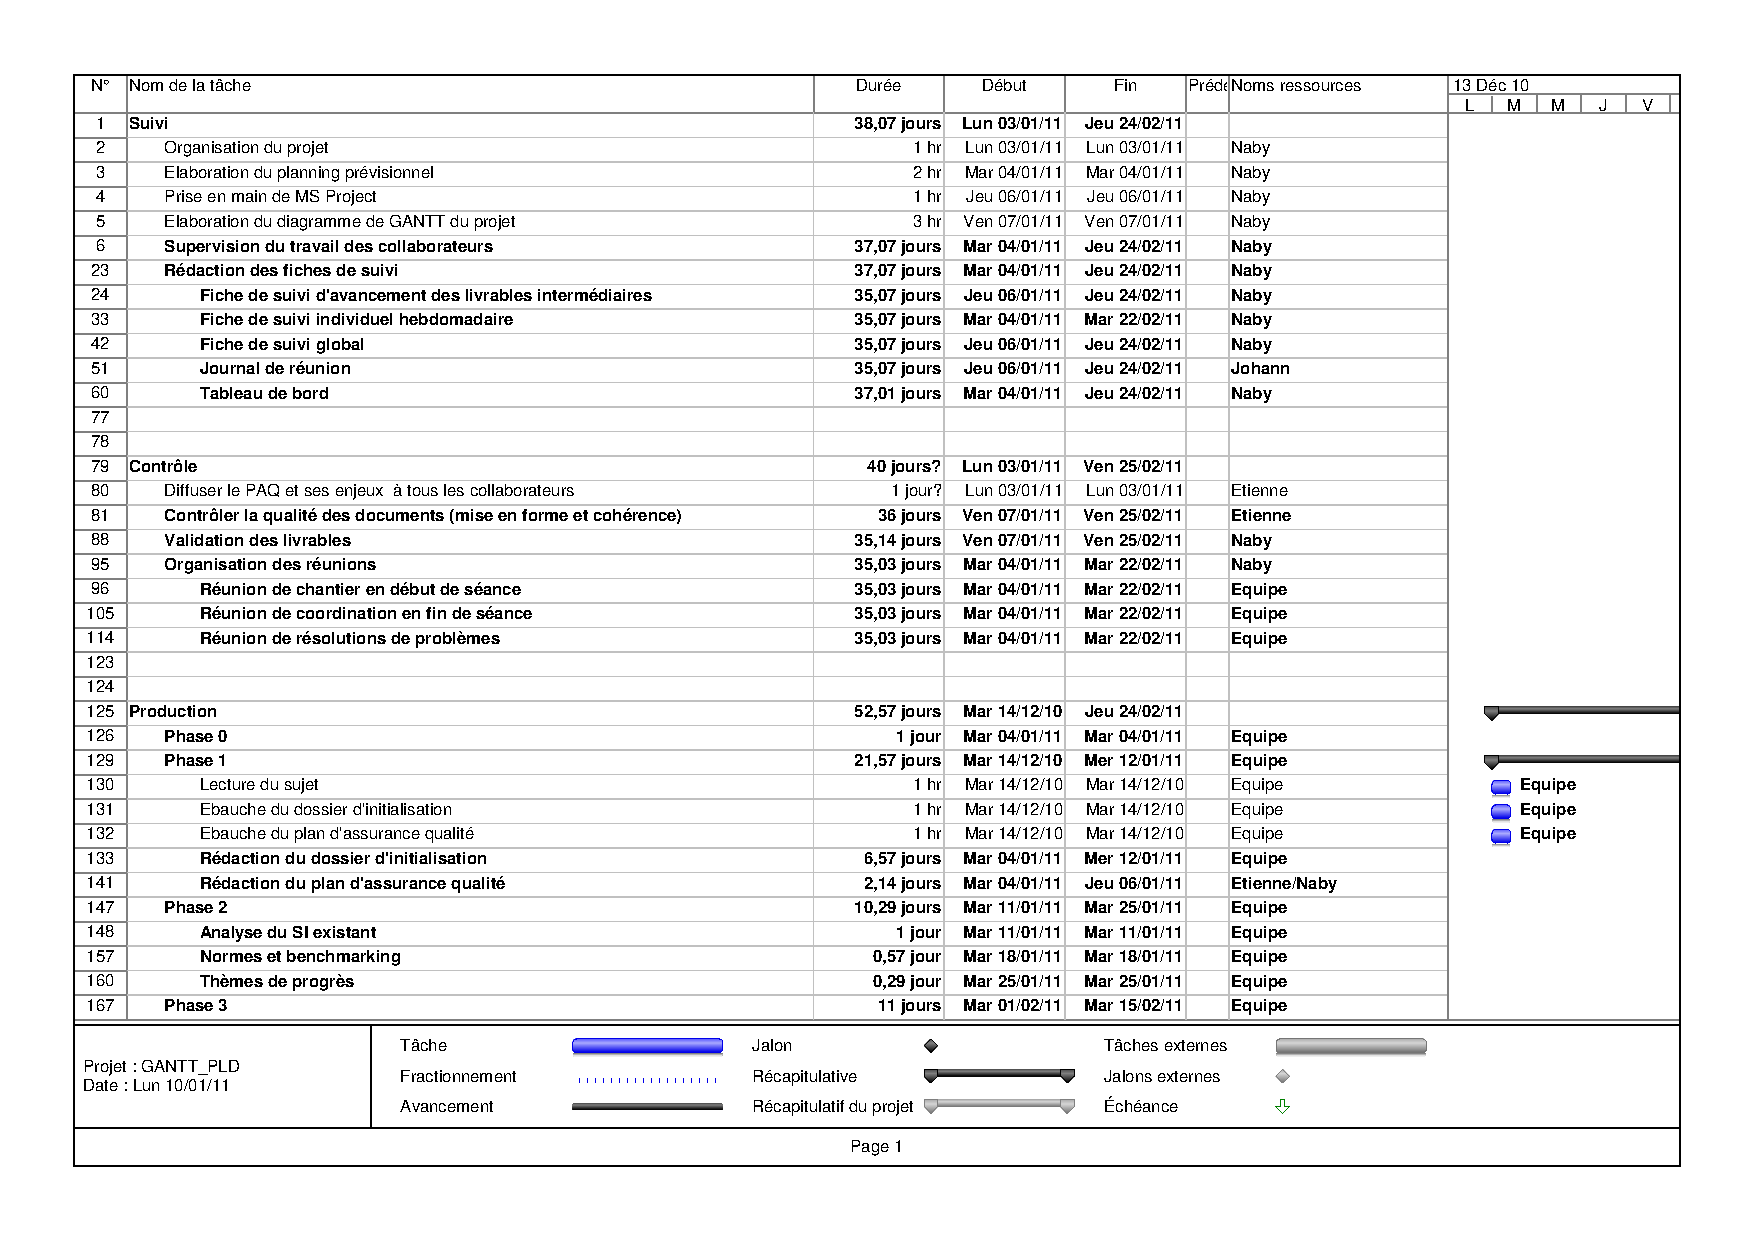
\includepdf[page=1]{img/gant.pdf}
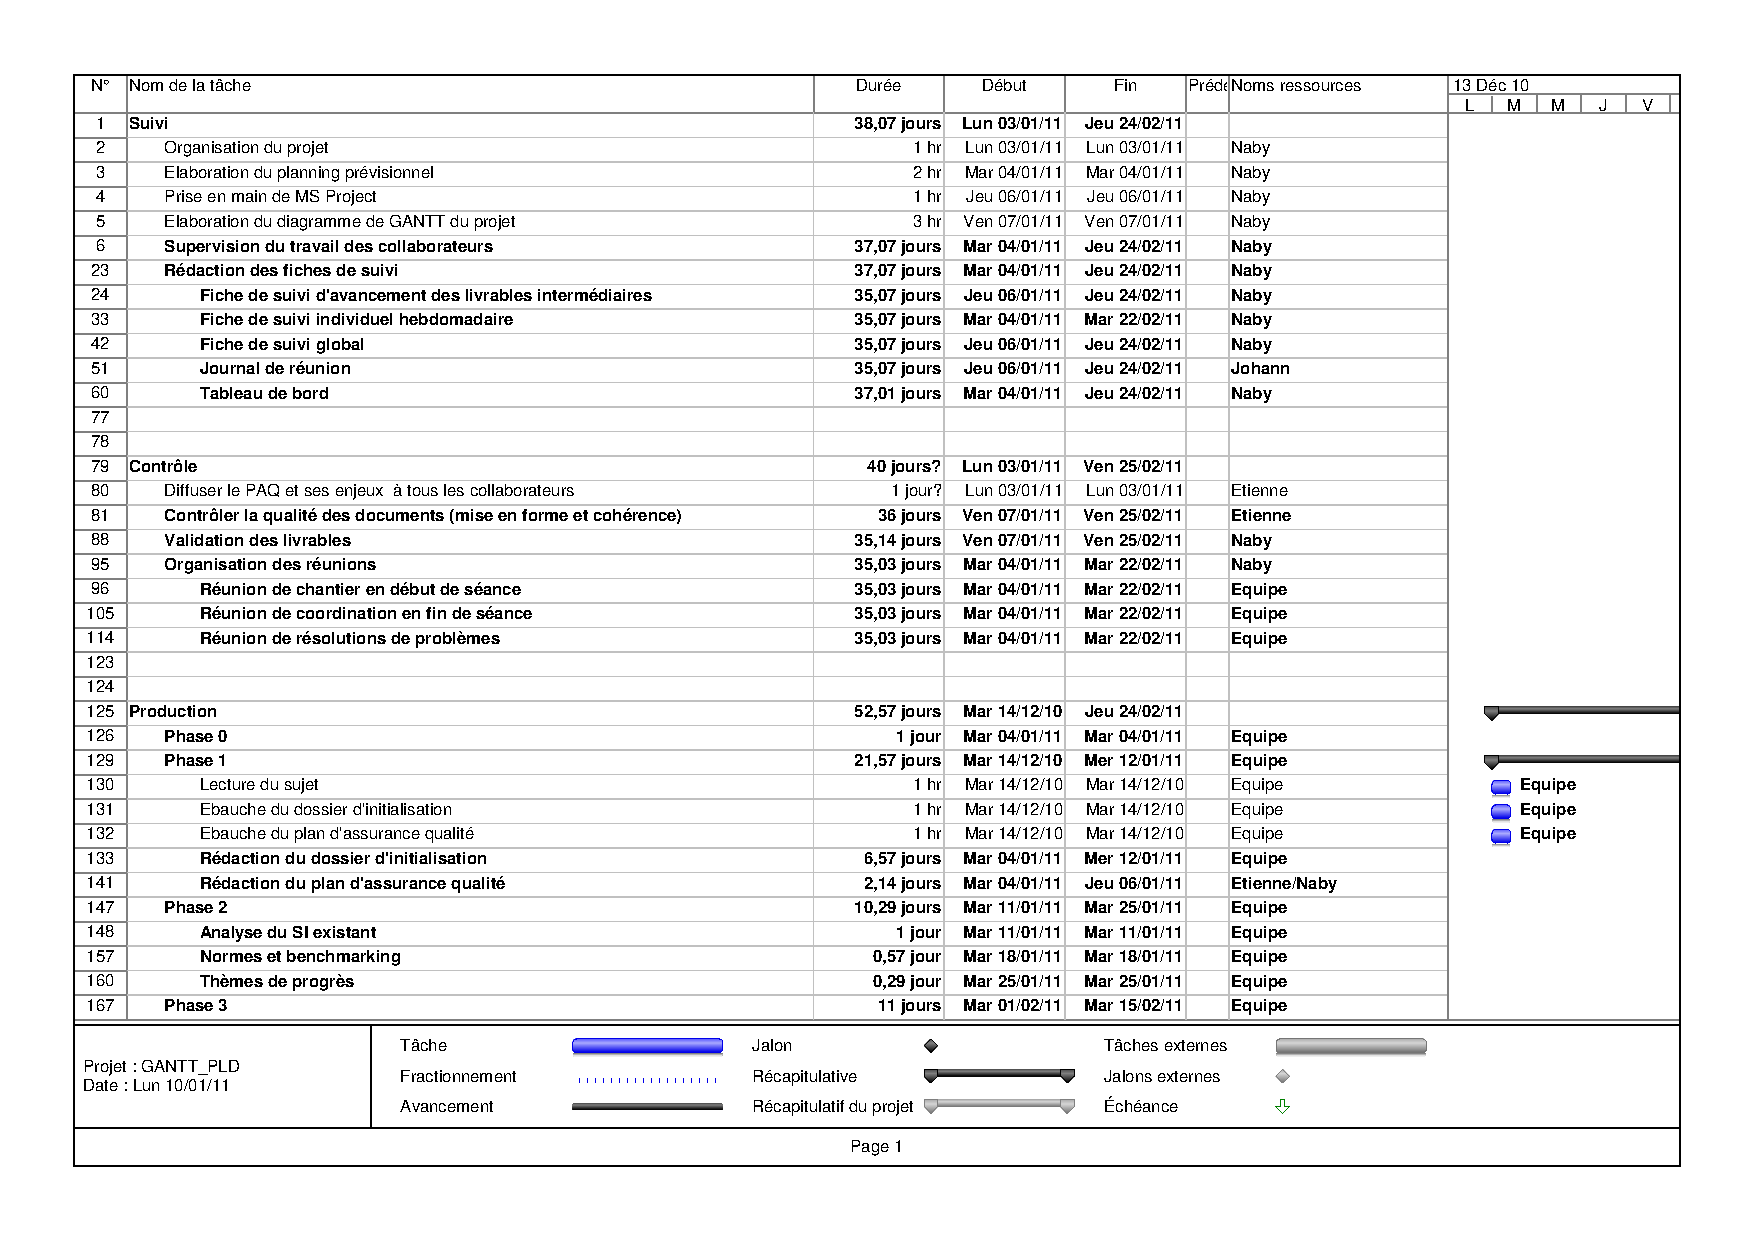
\includepdf[page=2]{img/gant.pdf}
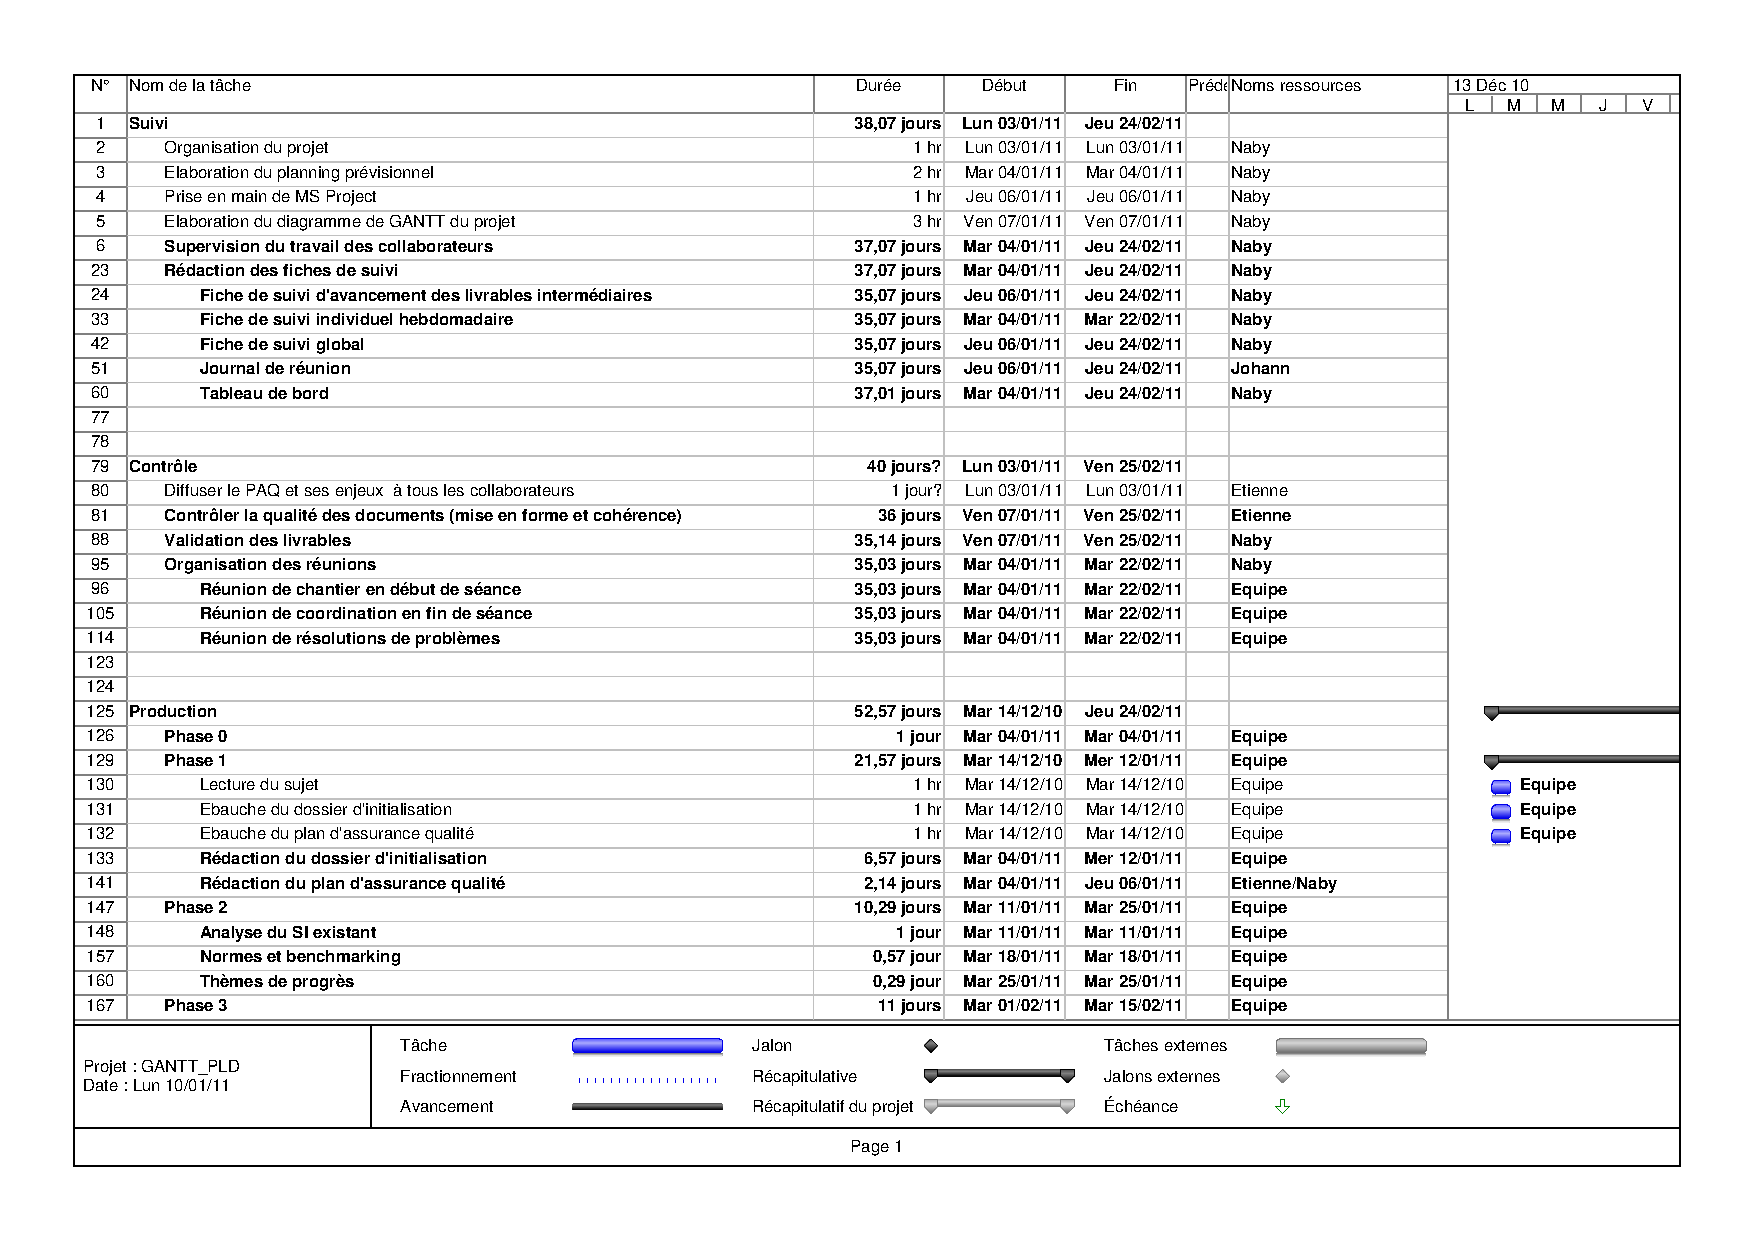
\includepdf[page=3]{img/gant.pdf}
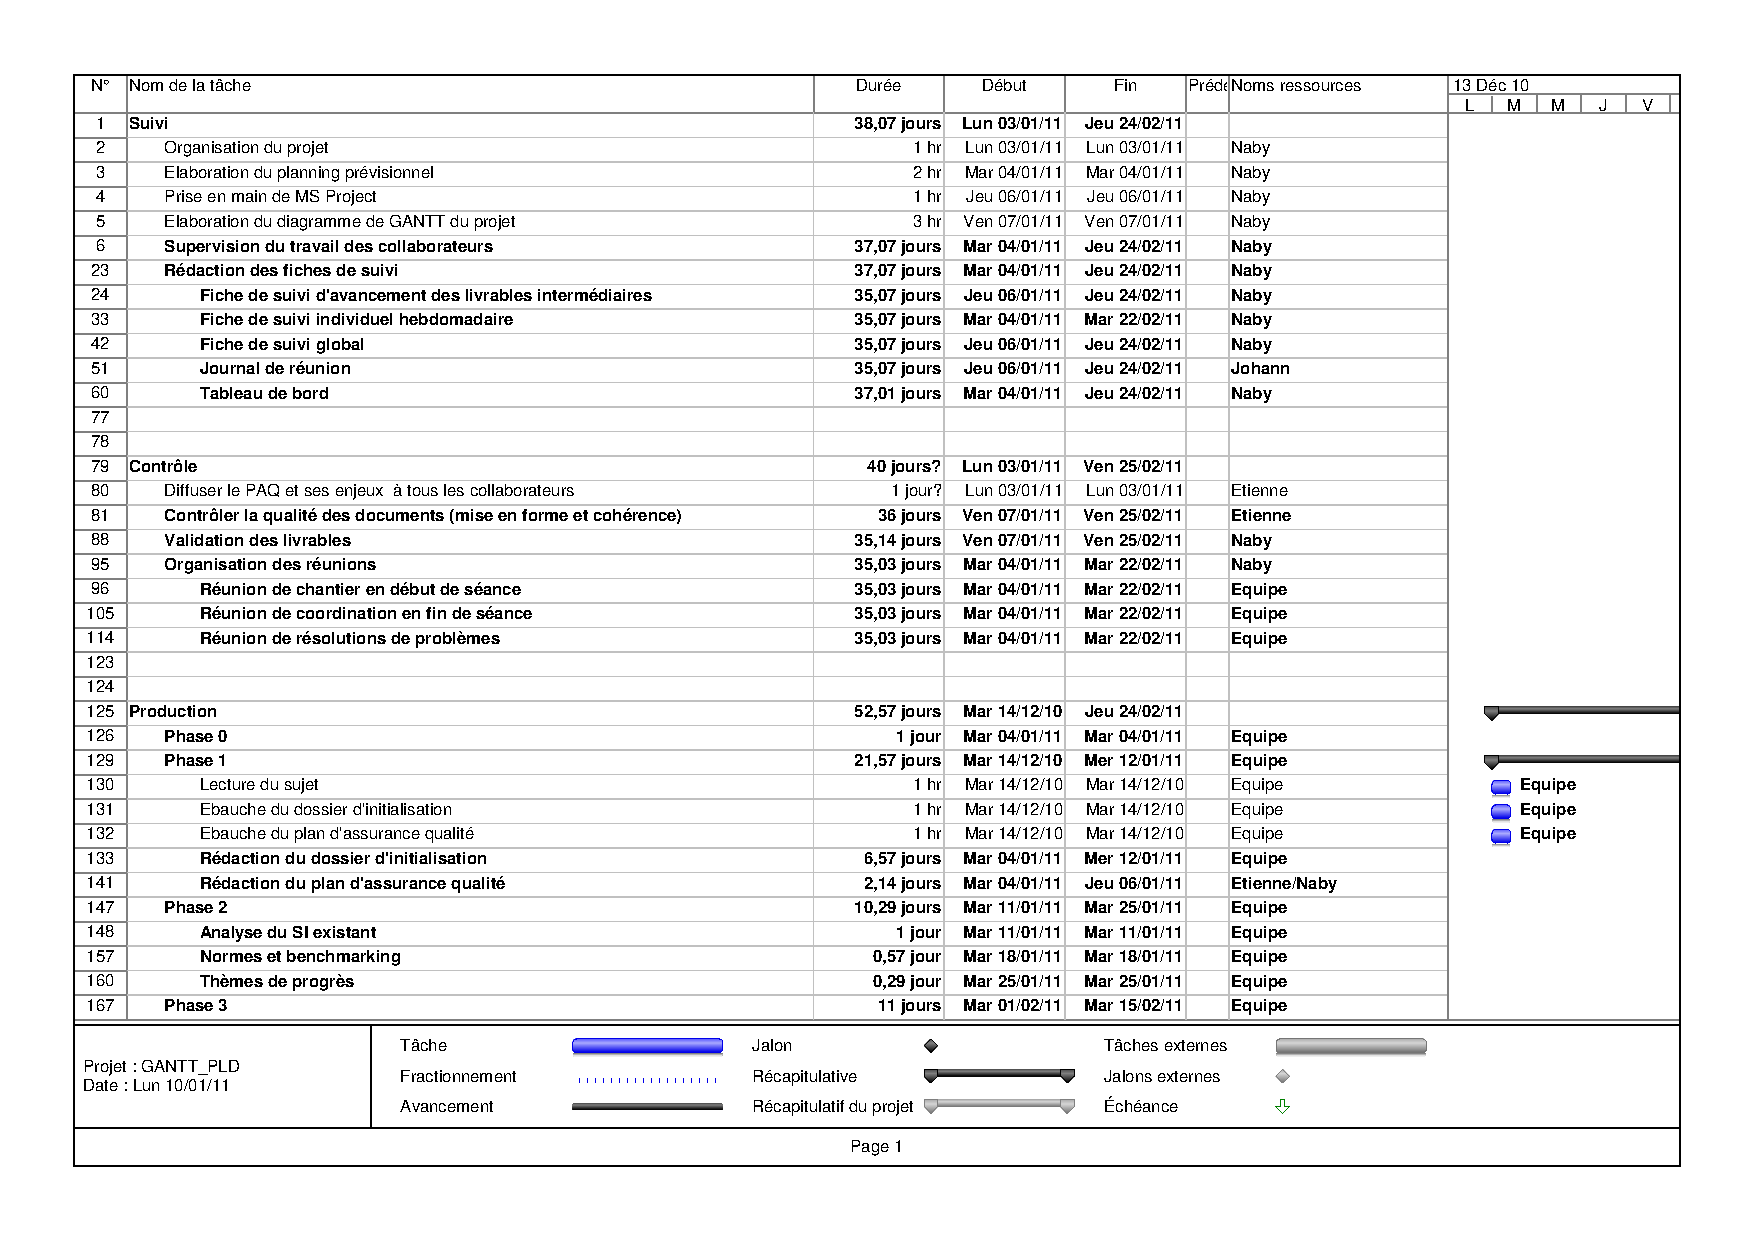
\includepdf[page=4]{img/gant.pdf}
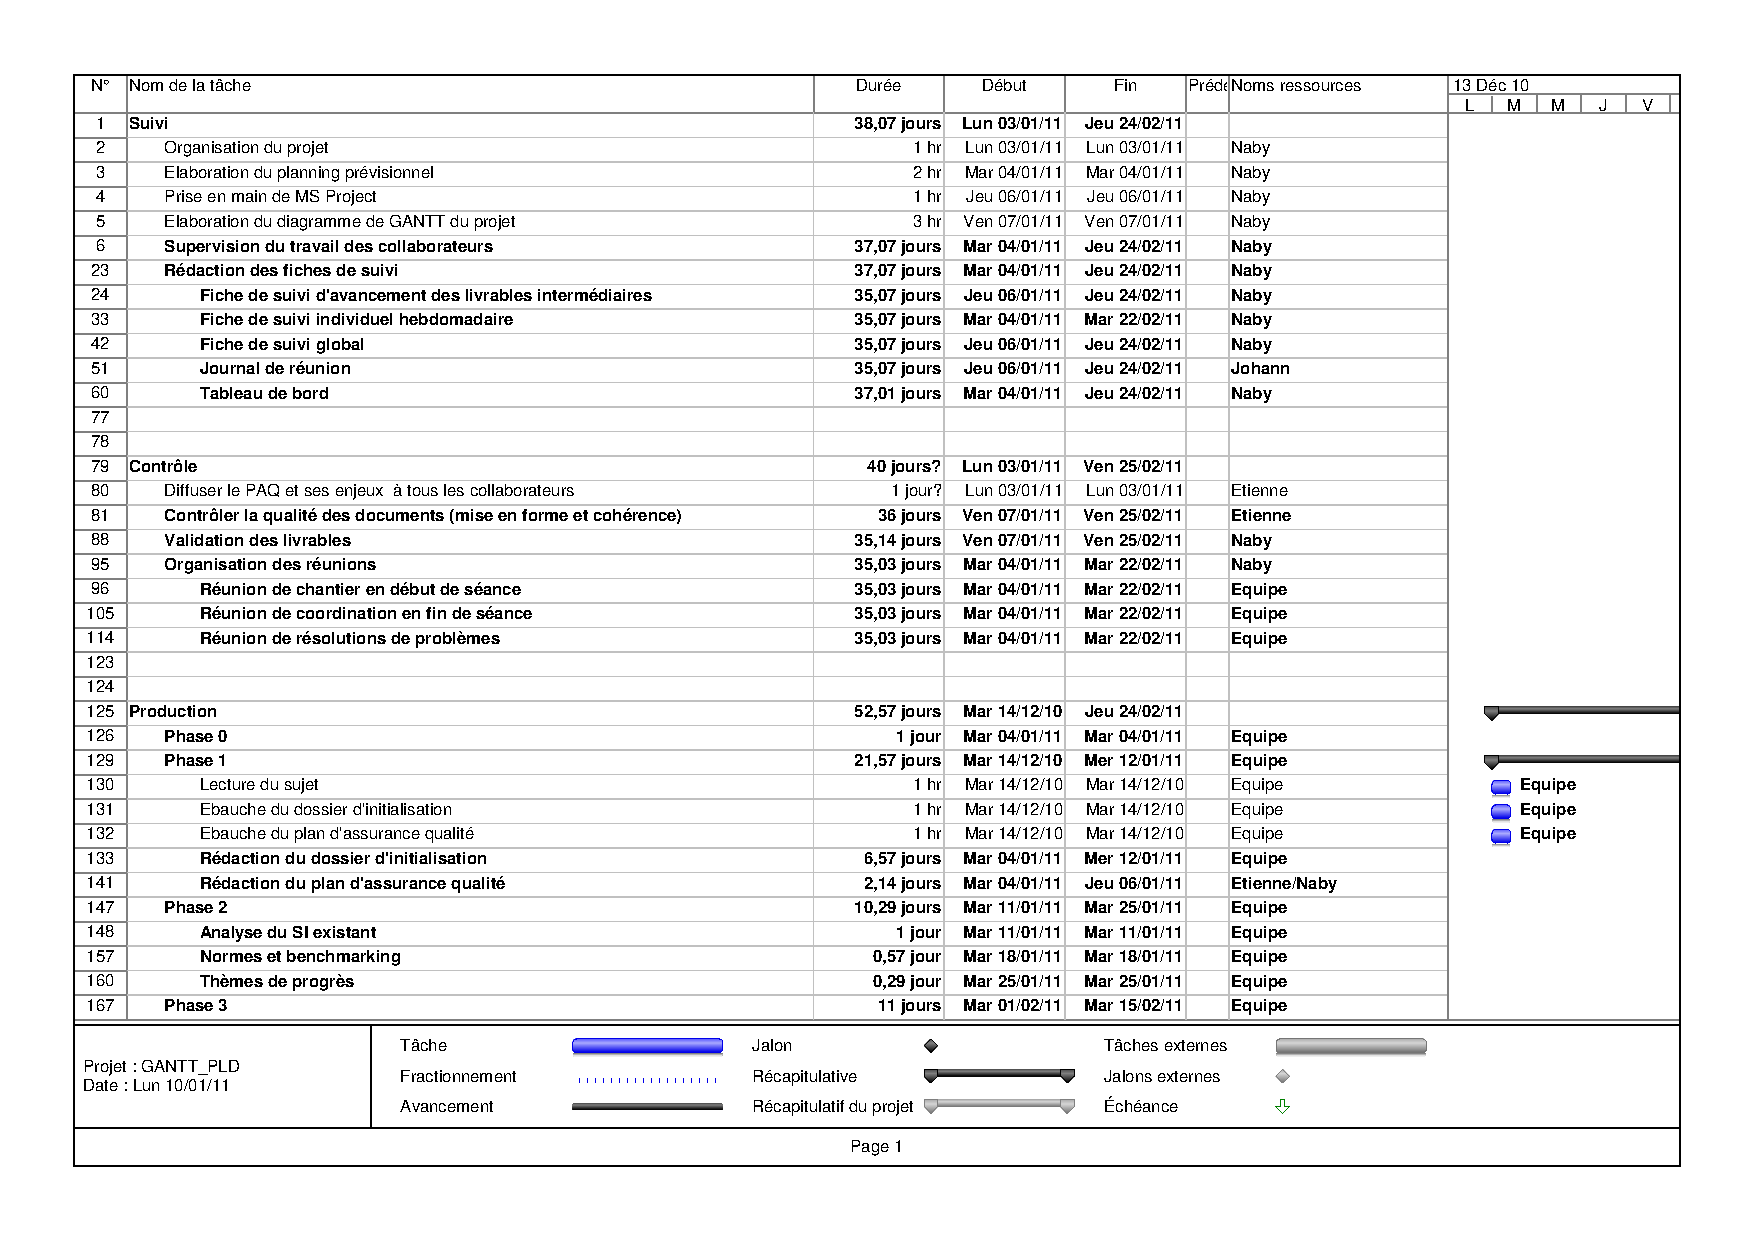
\includepdf[page=5]{img/gant.pdf}
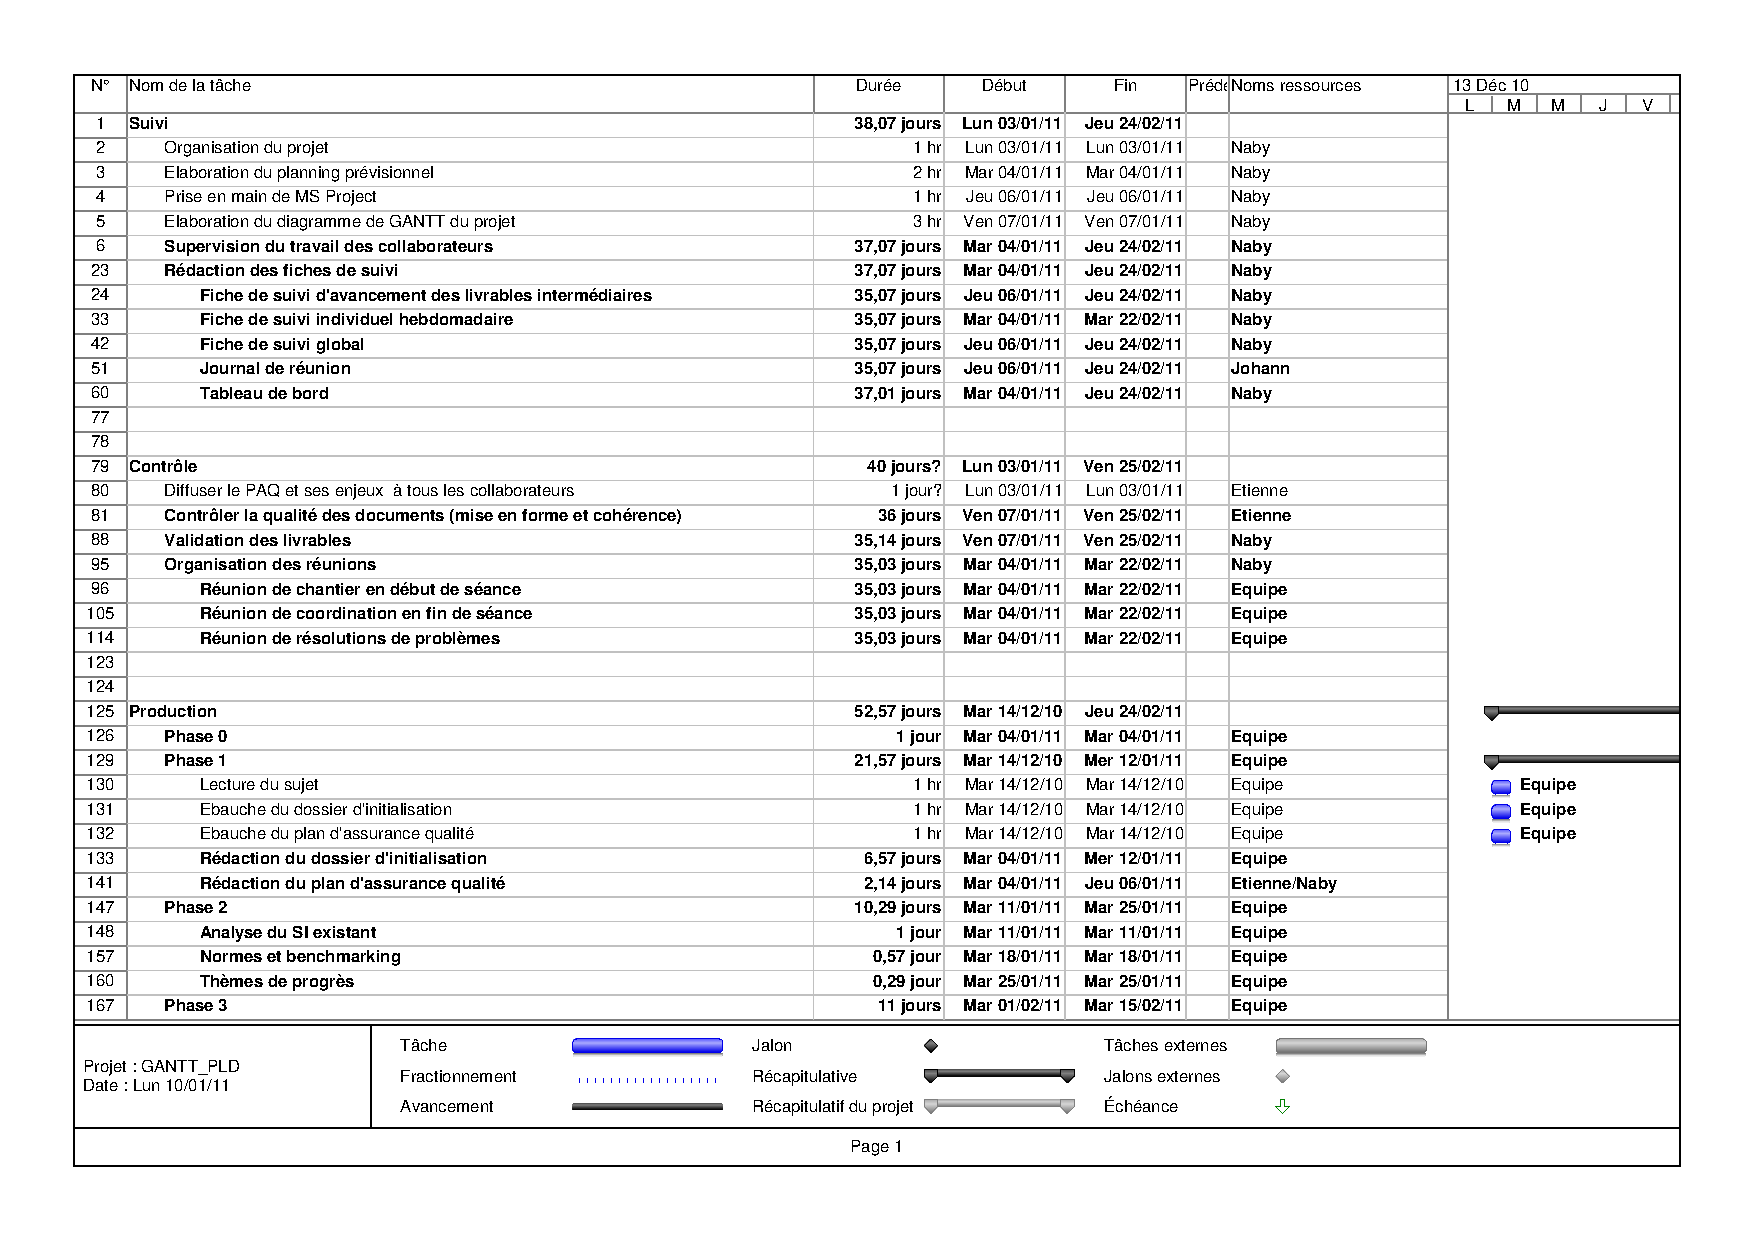
\includepdf[page=6]{img/gant.pdf}

\vspace{10 mm}

\section{Organisation de l'équipe}

L’équipe projet sera organisé ainsi :
\subsection{Chef de projet : Naby Daouda \textsc{Diakite}}

Son rôle sera :
\begin{itemize}
    \item Suivi stratégique du projet
        \subitem Évaluation risques
        \subitem Respect des objectifs
        \subitem Respects des délais
    \item Pilotage opérationnel
        \subitem Planification des taches
        \subitem Suivi et encadrement des tâches
    \item Organisation humaine
        \subitem Définition du rôle des membres et leur responsabilité
        \subitem Résolution de conflits et arbitrage
    \item Pilotage de la production
        \subitem Suivi des résultats et livrables
        \subitem Méthodes et outils
    \item Production des livrables
\end{itemize}

\subsection{Responsable qualité : Etienne \textsc{Brodu}}

Son rôle sera :
\begin{itemize}
    \item Charte qualité
    \item Cohérence entre les livrables
    \item Rédaction, MAJ  et Respect PAQ
    \item Production des livrables
\end{itemize}

\subsection{Responsable communication : Johann \textsc{Chazelle}}

Son rôle sera :
\begin{itemize}
    \item Communications internes et externes
    \item Compte rendu de réunions
    \item Recensement des difficultés des collaborateurs
    \item Production des livrables
\end{itemize}

\subsection{Expert ERP/Modélisation : Baptiste \textsc{Lecornu}}

Son rôle sera :
\begin{itemize}
    \item Analyse et Conception de l’architecture générale
    \item Aide à la Modélisation et configuration des solutions 
    \item Production livrable
\end{itemize}


\subsection{Expert Métier Achat : Chafik \textsc{Bachatene}}

Son rôle sera :
\begin{itemize}
    \item Connaissance des normes et benchmarks des ERP proposant une gestion des achats
    \item Identification des processus métiers d'achat
    \item Production livrable
\end{itemize}

\subsection{Expert Métier Gestion de matériels : Adrien \textsc{Bachatene}}

Son rôle sera :
\begin{itemize}
    \item Connaissance des normes et benchmarks des ERP proposant une gestion de matériels
    \item Identification des processus métiers de gestion de matériels
    \item Production livrable
\end{itemize}

\subsection{Expert Métier Maintenance : Thanh \textsc{Bachatene}}

Son rôle sera :
\begin{itemize}
    \item Connaissance des normes et benchmarks des ERP proposant une gestion de la maintenance
    \item Identification des processus métiers de gestion de la maintenance
    \item Production livrable
\end{itemize}

\section{Analyse des risques}
\subsection{Risques}

\newcounter{risques}
\setcounter{risques}{0}

\newcommand{\risque}[1]{
    \addtocounter{risques}{1}
    \item[R\therisques]{\indent#1}
}
Les risques sont les suivants :
\begin{description}
    \risque{Risque humains (liés aux compétence, absence, maladie..)}
    \risque{Apparition de tâches supplémentaires liées à la saisie des livrables ( rapport)}
    \risque{Difficulté d’évaluation du temps nécessaire à chaque tâche(prise en main des outils et méthodes utilisés,...)}
    \risque{Spécification incomplète des points à traiter}
    \risque{Risque de sur-qualité}
    \risque{Délais tendus}
    \risque{Demande régulière de modification durant l’élaboration des solutions}
\end{description}

\subsubsection{Gestion des risques}

\newcounter{solutions}
\setcounter{solutions}{0}

\newcommand{\solution}[1]{
    \addtocounter{solutions}{1}
    \item[S\thesolutions]{\indent#1}
}

Les solutions que nous préconisons sont :
\begin{description}
    \solution{
        \begin{itemize}
            \item Imposer un certain nombre de règles à suivre pour le bon déroulement du projet et veiller au respect de ceux-ci. Si nécessaire formaliser ces règles sous forme de “règlement intérieur”.
            \item Motiver suffisamment les membres de l’équipe  et répartir les tâches en fonction des profils et des compétences de chacun
            \item Redistribuer le travail du membre indisponible aux autres membres de l’équipe durant toute la durée de son indisponibilité.
        \end{itemize}}
    \solution{
        Prévoir des créneaux horaires (hors séance) pour la prise en main des outils utilisés  et la centralisation de façon efficace des différents livrables.}

    \solution{
        Contrôle du planning prévisionnel et mise à jour de celui-ci et si nécessaire réaffectation des tâches}
    \solution{
        S’adresser au client pour éclaircir les points flous}
    \solution{
        \begin{itemize}
            \item Contrôler de façon permanente l’avancement des tâches et les documents produit
            \item Maquettage
        \end{itemize}}
    \solution{
        \begin{itemize}
            \item Planification détaillée du projet avec un GANTT
            \item Suivi de l’avancement des livrables
        \end{itemize}}
    \solution{
        \begin{itemize}
            \item Seuil d’acceptation des modifications
            \item Report des modifications en fin de projet
            \item Gestion de versions
        \end{itemize}}
